% vim: spelllang=es

\chapter{Investigación previa}\label{sec:investigation}

La propuesta para el sistema de plugins asumía que se iba a implementar con un
método que cubriré posteriormente denominado \emph{cargado dinámico}. Esto se
debe a razones de rendimiento, pero el método también incluye otros problemas
importantes, principalmente relacionados con seguridad. Por ello, es una buena
idea considerar las alternativas existentes para el PDK, en caso de que hubiera
alguno con la misma eficiencia pero menos vulnerabilidades.

Los requerimientos mínimos a tener en cuenta son los siguientes:

\begin{itemize}
    \item Debe ser posible añadir y quitar plugins tanto en el inicio del
        programa como durante su ejecución.

    \item Disponibilidad y madurez en el ecosistema de Rust.

    \item Soporte multi-plataforma: Windows, MacOS y Linux.

    \item No debe tener un impacto excesivo en el rendimiento. Esto significa
        que los eventos no se pueden copiar en ningún momento.

\end{itemize}

Y opcionalmente:

\begin{itemize}
    \item Maximizar la seguridad en lo posible, como se especifica en la sección
        \ref{sec:security}.

    \item Debería ser retro-compatible con el código ya existente, como indica la
        sección \ref{sec:compat}.

    \item Minimizar el esfuerzo necesario para reescribir los conectores para el
        nuevo sistema de plugins.

\end{itemize}

\section{Seguridad}\label{sec:security}

\subsection{Código \unsafe}

Muchas de las tecnologías que se pueden aplicar para un sistema de plugins usan
código \unsafe. Técnicamente, esto no es necesariamente un problema si la
implementación está autocontenida y auditada exhaustivamente, pero se pierden
algunas garantías que proporcionadas por Rust, incrementando el coste de
mantenimiento de la librería.

Asegurarse de que la implementación es segura implica una cantidad
considerablemente mayor de trabajo, aun cuando existen herramientas como
MIRI\footnote{\url{https://github.com/rust-lang/miri}} --- que integraría en
Tremor en caso de tener que recurrir a \unsafe.

\subsection{Resiliencia a errores}

Rust no protege a sus usuarios de \leaks de memoria. De hecho, es tan sencillo
como llamar a \code{mem::forget}. Si un plugin tuviera un \leak, el proceso
entero también se vería afectado; el rendimiento de Tremor se degradaría con
plugins no desarrollados incorrectamente. Algo similar podría suceder en caso de
que un plugin abortase o sufriese de un \panic, lo que terminaría la ejecución
del programa por completo.

Idealmente, Tremor debería poder detectar plugins que no rinden óptimamente y
pararlos antes de que sea demasiado tarde. La runtime debería poder continuar
corriendo aun cuando falle un plugin, posiblemente avisando al usuario o
reiniciándolo para seguir funcionando.

\subsection{Ejecución de código remota a través de plugins}

Uno de los casos más notorios se dio con Internet Explorer, que usaba COM y
ActiveX, los cuales no disponían de una \sandbox. Dicho mecanismo aisla por
completo parte del programa, de forma que no pueda acceder a memoria externa
(evitando acceder a información que no es suya), ni a recursos del sistema (como
ficheros). Por tanto, extensiones maliciosas para el navegador podían ejecutar
código arbitrario en la máquina en la que estuviera instalado~\cite{iesandbox}.
Este problema puede ser menos grave si solo se instalan extensiones de confianza
con firmas digitales, pero sigue siendo un vector de ataque importante.

Se podría aplicar lo mismo a Tremor. El usuario del producto --- aquellos que
añadan plugins a su configuración ---, es un desarrollador, que debería ser más
consciente sobre lo que incluye en sus proyectos. Sin embargo, en la práctica
esto no es cierto.

Podría compararse con cómo funcionan los administradores de paquetes como
npm\footnote{\url{https://www.npmjs.com/}}. Su infraestructura se suele basar
por completo en cadenas de confianza; no hay nadie que te impida crear un
paquete malicioso para ejecutar código remoto o robar
credenciales~\cite{npm1}\cite{npm2}. Los plugins son como dependencias en este
caso; tienen acceso completo a la máquina donde se ejecutan, y por tanto no
deberían ser de confianza por defecto.

% TODO: puedo usar expresiones como 'terreno pantanoso' o es demasiado informal?
Una alternativa mejorada a Node y npm sería algo como
Deno\footnote{\url{https://github.com/denoland/deno}}, que es una runtime segura
por defecto. Esto es posible gracias a \sandboxing, y requiere que el
desarrollador active manualmente, por ejemplo, acceso al sistema de ficheros o a
la red. No es una solución infalible porque puede que los desarrolladores acaben
activando los permisos que necesitan sin pensarlo, pero es un mecanismo similar
a \unsafe: al menos te hace consciente de que estás en terreno pantanoso.

Se podría discutir que, realísticamente, el programa va a ejecutarse la mayoría
de los casos en una máquina virtual o un contenedor, donde este problema no es
tan peligroso. Pero, ¿debería la seguridad del usuario recaer en el hecho de que
el kernel está isolado? Por no mencionar que un contenedor afecta mucho más al
rendimiento que algunos métodos de \sandboxing. Aunque el sistema por completo
estuviera isolado, seguiría habiendo una posibilidad de \leaks internos: el
plugin de Postgres tiene acceso a todo lo que esté usando el plugin de Apacha
Kafka, que posiblemente tenga \emph{logs} sensitivos.

\section{Retro-compatibilidad}\label{sec:compat}

Será necesario incluir algún tipo de gestión de versiones en el proyecto. Es
probable que la interfaz de Tremor cambie con frecuencia, lo que romperá plugins
basados en versiones previas. Si un plugin recibe una estructura de la runtime,
pero esta estructura perdiese uno de sus campos en una nueva versión, se estará
invocando comportamiento no definido.

\subsection{Posibles soluciones}

La idea más sencilla para arreglar problemas con retrocompatibilidad es
serializar y deserializar los datos con un protocolo flexible, en vez de usando
su representación binaria directamente. Si se usara un protocolo como JSON para
comunicarse entre la runtime y los plugins, añadir un campo no rompería nada, y
eliminar uno puede ocurrir mediante un proceso de deprecación. Por desgracia,
esto implicaría una degradación en el rendimiento que posiblemente no interese
en la aplicación. Otros arreglos más elaborados para representaciones binarias
incluyen~\cite{swiftabi}:

\begin{itemize}
    \item Reservar espacio en la estructura para uso futuro.

    \item Hacer la estructura un tipo opaco, es decir, que sólo se puede acceder
        a sus campos con llamadas a funciones, en lugar de directamente.

    \item Dar a la estructura un puntero a sus datos en la ``segunda versión''
        (lo cual sería opaco en la ``primera versión'').

\end{itemize}

\subsection{Evitar errores}

Hay casos donde un error inevitable. Es posible que Tremor quiera reescribir
parte de su interfaz o finalmente eliminar una funcionalidad deprecada sin tener
que preocuparse por romper todos los plugins desarrollados previamente.

Para ello, los plugins deben incluir metadatos sobre las diferentes versiones
de rustc/interfaz/etc para las que fue desarrollado. Después, cuando sean
cargados por Tremor, se podrá comprobar su compatibilidad, en vez de romperse de
formas misteriosas.

\section{Tecnologías a considerar}

Esta sección describe las tecnologías que se han considerado más viables como
base para el PDK. Algunas de ellas no cumplirán los requerimientos mencionados
al principio del capítulo, pero es necesario aprender sobre ellas primero antes
de escribir ninguna línea de código.

\subsection{Lenguajes interpretados}

Todo tipo de proyectos usan lenguajes interpretados para extender su
funcionalidad a tiempo de ejecución, como Python, Ruby, Perl, Bash, o
JavaScript. Particularmente, el editor de texto Vim creó su propio lenguaje para
poderlo personalizar por completo, Vimscript. Ahora NeoVim, una alternativa más
moderna, está esforzándose por tener Lua como lenguaje de primera clase para su
configuración. Incluso Tremor tiene su propio lenguaje para configurarlo, Troy.

% TODO: existe 'embeber' (traducción de embed) o me lo he inventado?
Lua es popular en desarrollo de videojuegos; es un lenguaje simple con una
implementación \emph{Just-In-time} (JIT) de muy alto rendimiento, por lo que
sería de las mejores opciones para Tremor. Se podría embeber en la runtime, dado
que solo ocupa 247kB compilado~\cite{luawhy}.

\subsection{Comunicación Inter-Proceso}

\begin{figure}
    \centering
    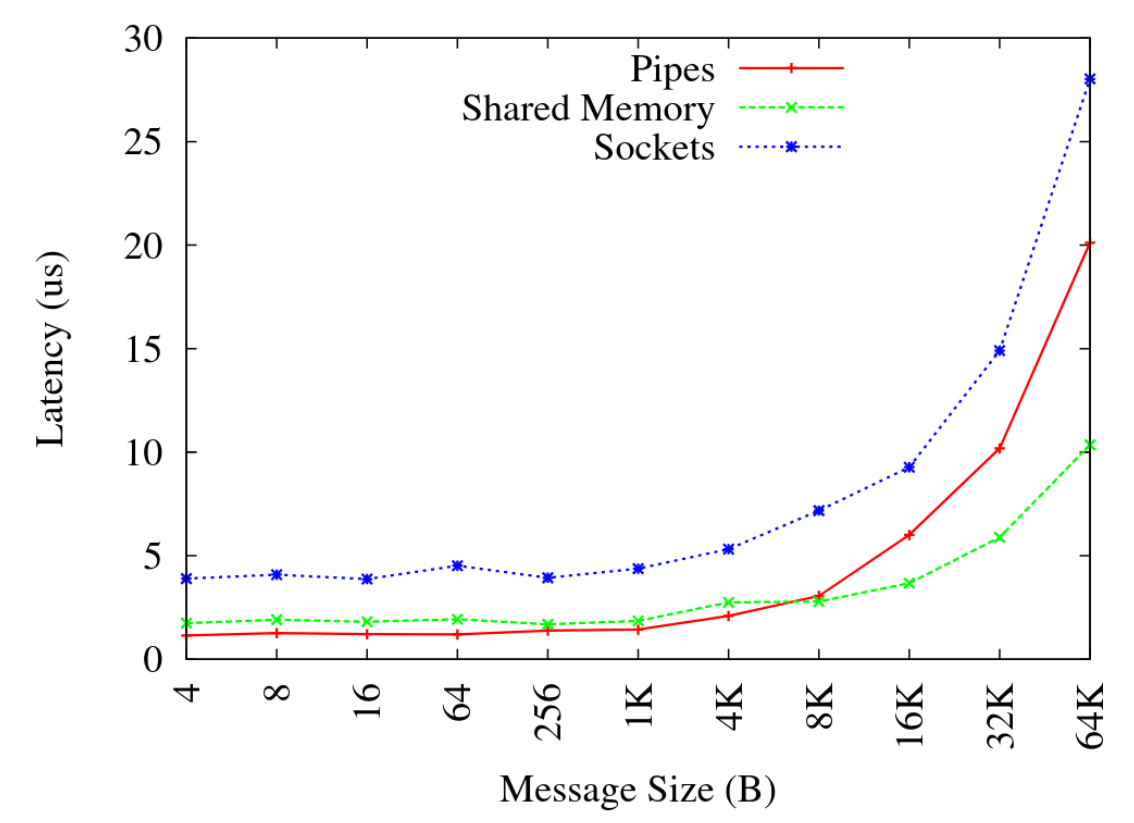
\includegraphics[width=10cm]{./Imagenes/venkataraman2015evaluation1.png}
    \caption{Latencia vs. Tamaño de Mensaje \cite{venkataraman2015evaluation}}%
    \label{fig:ipc_comparison1}
\end{figure}

\begin{figure}
    \centering
    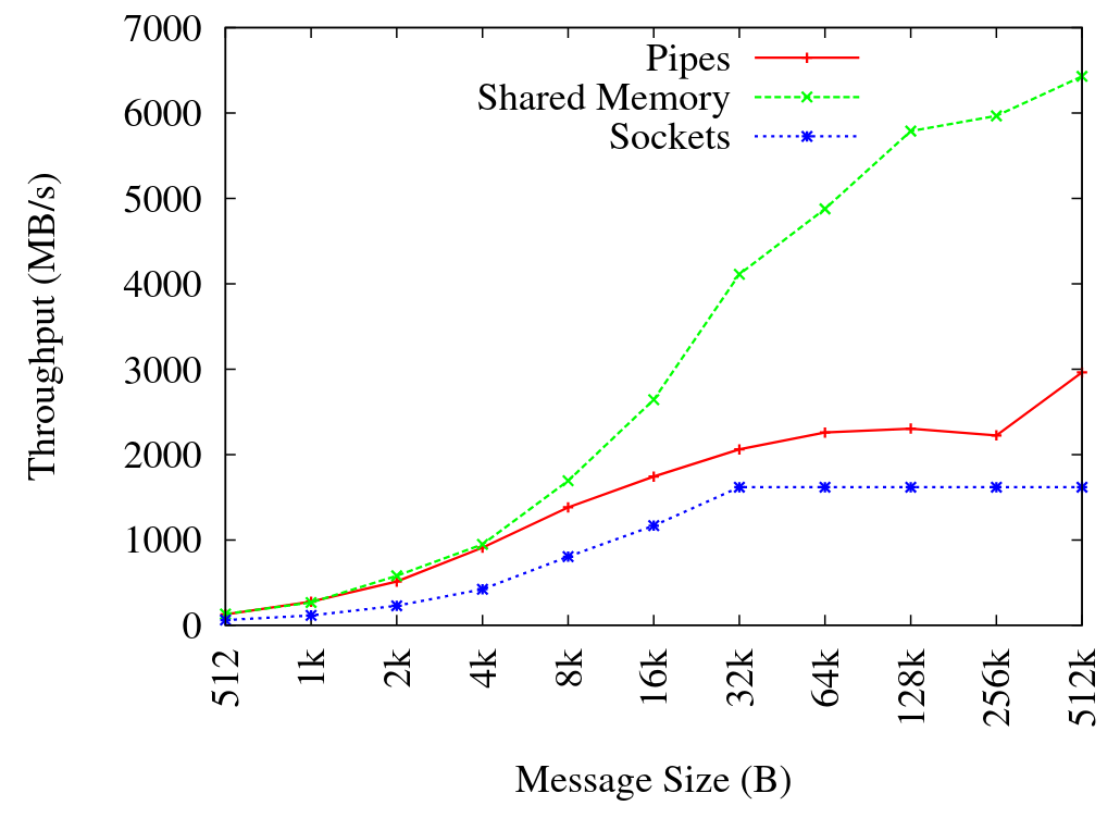
\includegraphics[width=10cm]{./Imagenes/venkataraman2015evaluation2.png}
    \caption{Rendimiento vs. Tamaño de Mensaje \cite{venkataraman2015evaluation}}%
    \label{fig:ipc_comparison2}
\end{figure}

\subsection{Cargado dinámico}

\subsection{WebAssembly}

\subsection{eBPF}

\section{Conclusión}

\begin{figure}
    \centering
    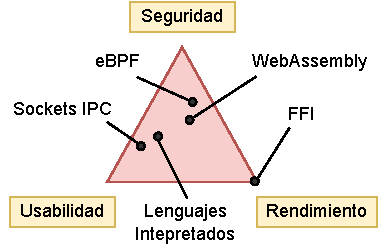
\includegraphics[width=10cm]{./Imagenes/triangle.pdf}
    \caption{Ejemplo de uso de Tremor}%
    \label{fig:tech_triangle}
\end{figure}
